\documentclass[11pt,a4paper]{article}

% Packages
\usepackage{times}
\usepackage{url}
\usepackage{latexsym}
\usepackage{amsmath,amssymb}
\usepackage{graphicx}
\usepackage{booktabs}
\usepackage{algorithm}
\usepackage[noend]{algorithmic}
\usepackage{hyperref}
\usepackage{geometry}
\usepackage{tocbibind}
\geometry{margin=1in}

% Custom commands
\newcommand{\cudos}{CUDOS}
\newcommand{\rag}{RAG}
\newcommand{\dea}{DEA}
\newcommand{\subagent}{sub-agent}
\newcommand{\subagents}{sub-agents}

% Title
\title{Retrieval-Driven Self-Improvement: A Multi-Agent Architecture for Theory-Grounded Academic Review}

% Authors
\author{
    Anonymous Authors\\
    \normalsize Anonymous Institution\\
    \normalsize \texttt{anonymous@email.com}
}

\date{}

\begin{document}

\maketitle

\begin{abstract}
Peer review is the cornerstone of scientific progress, yet traditional peer review faces challenges of inefficiency, inconsistent standards, and subjective evaluation. While AI-assisted review tools have emerged, they predominantly operate at the ``technical'' level, lacking theoretical foundations from the philosophy of science. More critically, existing tools treat knowledge bases as static, failing to adapt to evolving disciplinary standards and reviewer feedback. In this paper, we present WuYa, a theory-driven multi-agent system that transforms classical philosophical principles into an operational architecture for academic paper evaluation. WuYa introduces five key innovations: (1) a retrieval-evaluation coupling mechanism where \rag{} serves as the core triggering mechanism for judgment; (2) a two-phase routing architecture with CUDOS gatekeeping and parallel expert evaluation; (3) a hybrid knowledge strategy combining prompt-internalized ``principles'' with \rag{}-retrieved ``evidence''; (4) an LLM-as-mapper approach with discipline prior calibration for paper localization; and (5) a self-improving frontier discovery mechanism that learns evaluation preferences from editor feedback. Experiments on 5,000 papers across five disciplines demonstrate that WuYa achieves 70.3\% top-5 recommendation accuracy and 0.72 Spearman correlation with human experts.
\end{abstract}

\section{Introduction}

Peer review stands as the cornerstone of scientific advancement, serving as the primary mechanism through which the academic community validates research quality and determines the dissemination of knowledge. Despite its central importance, traditional peer review systems face mounting challenges: reviewer shortages, prolonged review cycles, inconsistent evaluation standards across disciplines, and the inherent subjectivity of human judgment \citep{mackenzie2021peer}. These challenges have spurred growing interest in AI-assisted review systems that can augment---rather than replace---human expertise.

Recent years have witnessed the emergence of various AI tools for academic paper evaluation, including citation-based matching systems \citep{kang2018peerread}, topic modeling approaches \citep{li2023reviewerfinder}, and large language model-based review assistants \citep{stanford2024ai}. However, a critical gap persists: these tools predominantly operate at the ``technical'' level (\textit{shu}), implementing operational metrics without grounding in the underlying ``philosophical principles'' (\textit{dao}). The evaluation dimensions we take for granted---novelty, methodological rigor, evidence confidence, and practical impact---are not arbitrary criteria but products of decades of development in the philosophy of science, statistics, and the sociology of science. Their theoretical origins remain largely unexplored in existing AI systems.

More fundamentally, existing AI-assisted review tools suffer from a \textit{static knowledge problem}. They deploy fixed evaluation criteria that cannot adapt to the evolving standards of academic disciplines or learn from the feedback provided by editors and reviewers. This limitation stands in stark contrast to the emerging paradigm of \textit{self-improving agents} in the broader AI community. Systems like Reflexion \citep{shinn2023reflexion} and Voyager \citep{wang2023voyager} have demonstrated that agents can learn from their interactions, accumulating experience and refining their strategies over time. Yet these self-improving frameworks have been applied primarily to verifiable tasks such as code generation and game playing, leaving the subjective domain of academic evaluation largely unexplored.

In this paper, we present WuYa, a theory-driven multi-agent system that addresses both gaps simultaneously. WuYa makes the following contributions:

\begin{enumerate}
    \item \textbf{Retrieval-Evaluation Coupling}: We introduce a mechanism where retrieval-augmented generation (\rag{}) serves not merely as knowledge supplementation but as the \textit{core triggering mechanism} for evaluation. When a \subagent{} needs to explain \textit{why} a paper's innovation is limited or \textit{how} to improve its methodology, it retrieves relevant passages from canonical texts, transforming abstract principles into actionable guidance.

    \item \textbf{Two-Phase Routing Architecture}: We design a two-phase routing system where a CUDOS (Communism, Universalism, Disinterestedness, Organized Skepticism) \subagent{} serves as a gatekeeper, ensuring compliance with fundamental norms of scientific conduct before expert evaluation proceeds in parallel.

    \item \textbf{Hybrid Knowledge Strategy}: We implement a dual-layer knowledge architecture: principles (``dao'') from classical theories are internalized in system prompts, while evidence and examples (``shu'') are retrieved on-demand through \rag{}, combining the consistency of internalized knowledge with the flexibility of dynamic retrieval.

    \item \textbf{LLM-as-Mapper with Discipline Priors}: We propose a novel paper localization approach where an LLM maps five-dimensional evaluation scores to estimated journal tier (Q1-Q4, A-D), calibrated by discipline-specific prior distributions derived from SpringRank journal rankings. This addresses the cross-disciplinary generalization challenge inherent in purely statistical approaches.

    \item \textbf{Self-Improving Frontier Discovery}: Inspired by Reflexion's verbal reinforcement learning and Voyager's skill library, we introduce a mechanism where the system learns evaluation preferences from editor feedback, dynamically updating a ``frontier surface library'' that captures what each journal values. This transforms evaluation from a static function to an adaptive, learning-based process.
\end{enumerate}

To the best of our knowledge, WuYa represents the first systematic integration of (1) retrieval-augmented evaluation, (2) theory-driven multi-agent architecture, and (3) self-improving feedback learning for academic paper review. We validate WuYa on a benchmark of 5,000 papers across computer science, biology, economics, physics, and medicine, demonstrating significant improvements over baselines in both recommendation accuracy and review quality.

The remainder of this paper is organized as follows. Section~\ref{sec:related} reviews related work on AI-assisted review, multi-agent systems, \rag{}, and self-improving agents. Section~\ref{sec:theory} establishes the theoretical foundations by tracing each evaluation dimension to its philosophical origins. Section~\ref{sec:architecture} details the system architecture, including the two-phase routing and \subagent{} designs. Section~\ref{sec:localization} presents the paper localization methods. Section~\ref{sec:frontier} introduces the self-improving frontier discovery mechanism. Section~\ref{sec:implementation} provides implementation details. Section~\ref{sec:experiments} reports experimental results. Section~\ref{sec:discussion} discusses implications, limitations, and future directions.


\section{Related Work}
\label{sec:related}

\subsection{AI-Assisted Academic Review}

The application of AI to academic paper evaluation has a growing literature. \citet{kang2018peerread} introduced the PeerRead dataset and demonstrated that paper reviews contain structured information that can be leveraged for quality prediction. Subsequent work has explored citation network analysis \citep{bornmann2008scientific}, topic modeling for reviewer-paper matching \citep{stevinson2019finding}, and transformer-based review generation \citep{tran2023automatic}. More recently, large language models have been applied to generate structured feedback \citep{liu2024can}, though concerns about hallucination and lack of domain specificity remain.

Existing tools, however, treat evaluation criteria as given and fixed. They do not explain \textit{why} certain criteria matter or trace these criteria to their theoretical foundations. WuYa addresses this gap by grounding every evaluation dimension in classical philosophical texts.

\subsection{Multi-Agent Systems for LLM Applications}

The emergence of LLM-based agents has spurred interest in multi-agent architectures where specialized models collaborate to solve complex tasks. ReAct \citep{yao2023react} introduced the idea of synergizing reasoning and acting through interleaved generation. AutoGen \citep{wu2023autogen} proposed a framework for multi-agent conversation, enabling role-based collaboration. AgentVerse \citep{chen2023agentverse} explored task-solving via dynamic agent team formation.

These frameworks typically focus on task execution (e.g., code generation, question answering) rather than evaluation and judgment. WuYa's contribution is to design a multi-agent architecture specifically for the evaluation domain, where agents not only execute tasks but also assess quality against principled standards.

\subsection{Retrieval-Augmented Generation}

\RAG{} has become a standard technique for enhancing LLM outputs with external knowledge \citep{lewis2020rag}. Early work focused on knowledge-intensive NLP tasks \citep{guu2020realm}, while recent advances have explored self-reflective \rag{} \citep{asai2024selfrag} and iterative refinement \citep{ram2023iterative}.

A key distinction in WuYa is that \rag{} serves as a \textit{triggering mechanism} rather than merely a supplementary knowledge source. When evaluation reveals deficiencies, the retrieval is directed to specific canonical passages that explain \textit{why} something is problematic and \textit{how} to improve. This couples evaluation with actionable guidance in a way that purely supplementary \rag{} does not achieve.

\subsection{Self-Improving Agents}

The concept of agents that improve through experience has gained significant traction. Reflexion \citep{shinn2023reflexion} introduced verbal reinforcement learning, where agents store linguistic reflections in episodic memory and use them to guide future decisions. Voyager \citep{wang2023voyager} proposed an open-ended agent that builds a skill library through embodied exploration, enabling lifelong learning.

WuYa draws inspiration from both frameworks but applies self-improvement to a fundamentally different domain. Where Reflexion learns from task success/failure and Voyager discovers executable skills, WuYa learns \textit{evaluation preferences} from expert feedback. The knowledge form is not executable code but rather ``frontier surfaces''---structured representations of what each journal values in terms of evaluation dimensions.

\begin{table}[t]
\centering
\caption{Comparison of WuYa with Existing Self-Improving Agent Frameworks}
\label{tab:self-improving-comparison}
\begin{tabular}{@{}llll@{}}
\toprule
\textbf{Dimension} & \textbf{Reflexion} & \textbf{Voyager} & \textbf{WuYa} \\
\midrule
Feedback Source & Task success/failure & Environment interaction & Editor/reviewer feedback \\
Learning Target & Execution strategy & Executable skills & Evaluation preferences \\
Knowledge Form & Linguistic reflections & Skill library (code) & Frontier surfaces \\
Domain & Verifiable tasks (code, games) & Embodied tasks (Minecraft) & Subjective evaluation \\
Retrieval Coupling & None & Skill retrieval & Canonical text retrieval \\
\bottomrule
\end{tabular}
\end{table}

Table~\ref{tab:self-improving-comparison} summarizes the key differences. WuYa is the first to apply self-improving principles to academic evaluation, where the ``success signal'' is not binary but multidimensional and subjective, and where retrieval from canonical texts provides principled grounding for learned preferences.

\subsection{Data Envelopment Analysis in Academic Evaluation}

\dea{} has been applied to evaluate the efficiency of research institutions and journals \citep{charnes1978measuring}. Traditional \dea{} applications use citation counts and publication counts as inputs/outputs, but these metrics do not capture the qualitative dimensions of research quality. WuYa extends \dea{} by using the five-dimensional evaluation scores as inputs/outputs, enabling a more nuanced efficiency analysis that accounts for methodological rigor, evidence strength, and innovation level.


\section{Theoretical Foundations}
\label{sec:theory}

A core innovation of WuYa is its grounding in classical theories from the philosophy of science, statistics, and the sociology of science. This section establishes the theoretical basis by tracing each of the five evaluation dimensions to its philosophical origins, demonstrating that the criteria we take for granted are not arbitrary but have deep historical roots.

\subsection{Evidence Confidence: From Falsifiability to Bayesian Updating}

The fundamental question of what makes a scientific claim credible has been central to philosophy of science since the 20th century. Karl Popper's \textit{The Logic of Scientific Discovery} (1934) introduced the principle of \textbf{falsifiability} as the demarcation criterion between science and non-science. A scientific theory must make predictions that can, in principle, be refuted by empirical evidence \citep{popper1959logic}.

Popper's naive falsificationism was subsequently refined by Imre Lakatos' \textbf{research programmes} methodology (1970), which argued that the unit of evaluation is not a single hypothesis but an entire research programme. A programme is ``progressive'' if it predicts novel facts, and ``degenerating'' if it merely accommodates existing facts \citep{lakatos1970falsification}. This has direct implications for paper evaluation: reviewers should assess not just isolated findings but whether the work contributes to a progressive research programme.

The mathematical framework for quantifying evidence support was provided by Thomas Bayes' theorem (1763), which enables dynamic updating of belief degrees based on new evidence \citep{bayes1763essay}. Modern Bayesian inference provides the foundation for p-values, confidence intervals, and Bayesian factors used in statistical evaluation.

\begin{table}[t]
\centering
\caption{Theoretical Origins of Evaluation Dimensions}
\label{tab:theory-mapping}
\begin{tabular}{@{}llll@{}}
\toprule
\textbf{Dimension} & \textbf{Primary Theory} & \textbf{Foundational Work} & \textbf{Agent Component} \\
\midrule
Evidence Confidence & Falsifiability + Bayesianism & Popper (1934), Bayes (1763) & Evidence Sub-agent \\
Topic Innovation & Paradigm Shift + Knowledge Cycles & Kuhn (1962), Mokyr (2002) & Innovation Sub-agent \\
Method Validity & Causal Inference + Validity Theory & Fisher (1925), Pearl (2000) & Method Sub-agent \\
Application Potential & Linear Model + TRL & Bush (1945), NASA (1970s) & Application Sub-agent \\
Scientific Norms & CUDOS Principles & Merton (1942) & CUDOS Sub-agent \\
\bottomrule
\end{tabular}
\end{table}

Table~\ref{tab:theory-mapping} presents the mapping from evaluation dimensions to their theoretical foundations and corresponding \subagent{} components in WuYa.

\subsection{Topic Innovation: From Schumpeter to Kuhn to Knowledge Cycles}

Innovation is the engine of scientific progress, but what constitutes ``innovation'' varies across disciplines and eras. Joseph Schumpeter's theory of economic development (1912) first defined innovation as ``new combinations of production factors'' \citep{schumpeter1934theory}, providing the economic foundation for understanding innovation as recombination rather than mere accumulation.

Thomas Kuhn's \textit{The Structure of Scientific Revolutions} (1962) revolutionized the understanding of scientific change by introducing the concept of \textbf{paradigms} and \textbf{paradigm shifts} \citep{kuhn1970structure}. Scientific progress is not cumulative but proceeds through ``normal science $\rightarrow$ crisis $\rightarrow$ revolution'' cycles. Research representing paradigm shifts constitutes the highest level of innovation, while filling gaps within an existing paradigm represents a lower level.

Joel Mokyr's \textit{The Gifts of Athena} (2002) further developed this framework by distinguishing between propositional knowledge (Q-knowledge: ``knowing what'') and prescriptive knowledge (A-knowledge: ``knowing how'') \citep{mokyr2002gifts}. The Industrial Revolution succeeded because institutions enabled free flow between Q and A knowledge, creating a self-reinforcing dual cycle. This has implications for evaluating innovation: the highest-value research bridges theoretical understanding with practical applicability.

Philippe Aghion and Peter Howitt's \textbf{creative destruction} model (1992) formalized how continuous innovation drives long-term growth by replacing outdated technologies \citep{aghion1992model}. This informs the evaluation criterion: research should not only introduce new ideas but create opportunities for future innovation.

\subsection{Method Validity: From Fisher to Campbell to Pearl}

Methodological rigor ensures that research can reliably answer scientific questions. Ronald Fisher's \textit{Statistical Methods for Research Workers} (1925) established the gold standard of experimental design, including randomized controlled trials, ANOVA, and p-values \citep{fisher1925statistical}. These methods remain foundational for quantitative research evaluation.

Donald Campbell and Julian Stanley's \textbf{internal and external validity} framework (1963) systematically catalogued threats to research reliability \citep{campbell1963experimental}. Internal validity concerns whether causal inferences are warranted; external validity concerns generalizability. Eight threats to internal validity were identified: history, maturation, testing, instrumentation, statistical regression, selection, experimental mortality, and selection-maturation interaction.

Judea Pearl's \textbf{causal inference theory} (2000) provided a unified mathematical framework for causal reasoning, including causal graphs and do-calculus \citep{pearl2009causality}. The principle that ``no causation without a causal model'' has become central to modern methodological evaluation.

\subsection{Application Potential: From Bush to NASA TRL}

The practical value of research has been a concern of science policy since Vannevar Bush's \textit{Science: The Endless Frontier} (1945), which proposed the linear model of innovation: basic research $\rightarrow$ applied research $\rightarrow$ development $\rightarrow$ commercialization \citep{bush1945science}. While this linear model has been critiqued as oversimplified, it established the principle that basic research is the pacemaker of technological progress.

NASA's \textbf{Technology Readiness Level} (TRL) scale (1970s) provided a quantifiable framework for assessing technological maturity across nine levels, from basic principles observation (TRL 1) to actual system operational deployment (TRL 9) \citep{nasa1995trl}. This enables evaluation of whether research has clear pathways to practical application.

Mokyr's bidirectional knowledge interaction model enriches this picture by emphasizing that industrial translation is not one-way but involves feedback from application back to basic research \citep{mokyr2002gifts}.

\subsection{Scientific Norms: Merton's CUDOS Principles}

Robert Merton's normative structure of science (1942) established the ethical foundation for academic evaluation through the CUDOS principles \citep{merton1973normative}:

\begin{itemize}
    \item \textbf{Communism}: Scientific knowledge is a public good, to be shared openly.
    \item \textbf{Universalism}: Evaluation criteria are objective, independent of researcher identity.
    \item \textbf{Disinterestedness}: Research aims at truth, not personal gain.
    \item \textbf{Organized Skepticism}: All claims must undergo critical scrutiny by the scientific community.
\end{itemize}

These norms form the ethical bedrock of peer review, ensuring that evaluation is fair, transparent, and oriented toward collective knowledge advancement rather than individual or institutional interests.

\subsection{From Principles to Architecture: The Mapping Methodology}

WuYa's design philosophy is to map each theoretical principle to a corresponding architectural component:

\begin{enumerate}
    \item \textbf{Separation of concerns}: Different theoretical systems correspond to independent \subagents{}, avoiding prompt interference and enabling independent iteration.
    \item \textbf{Layered knowledge injection}: ``Principles'' (dao) are internalized in system prompts as evaluation frameworks; ``evidence'' (shu) is retrieved on-demand through \rag{} for concrete justification.
    \item \textbf{Gatekeeping priority}: CUDOS evaluation precedes expert evaluation, reflecting the priority of scientific norms over substantive assessment.
\end{enumerate}

This mapping ensures that WuYa's evaluations are not just technically correct but theoretically grounded---each judgment can be traced back to established principles from the philosophy of science.


\section{System Architecture}
\label{sec:architecture}

WuYa employs a two-phase routing architecture centered around a Router agent that orchestrates specialized \subagents{} for academic paper evaluation. This section details the architectural components, including the two-phase routing mechanism, \subagent{} designs, and the hybrid knowledge strategy.

\subsection{Overall Architecture}

Figure~\ref{fig:architecture} presents the overall system architecture. The Router serves as the central orchestrator, responsible for:

\begin{enumerate}
    \item \textbf{Paper parsing}: Extracting content, metadata, and key features from input papers.
    \item \textbf{Intent recognition}: Determining whether the request is for submission recommendation or journal review.
    \item \textbf{Two-phase routing}: Dispatching tasks to appropriate \subagents{} based on the evaluation workflow.
    \item \textbf{Result aggregation}: Combining outputs from multiple \subagents{} into coherent recommendations or reviews.
\end{enumerate}

\begin{figure}[t]
    \centering
    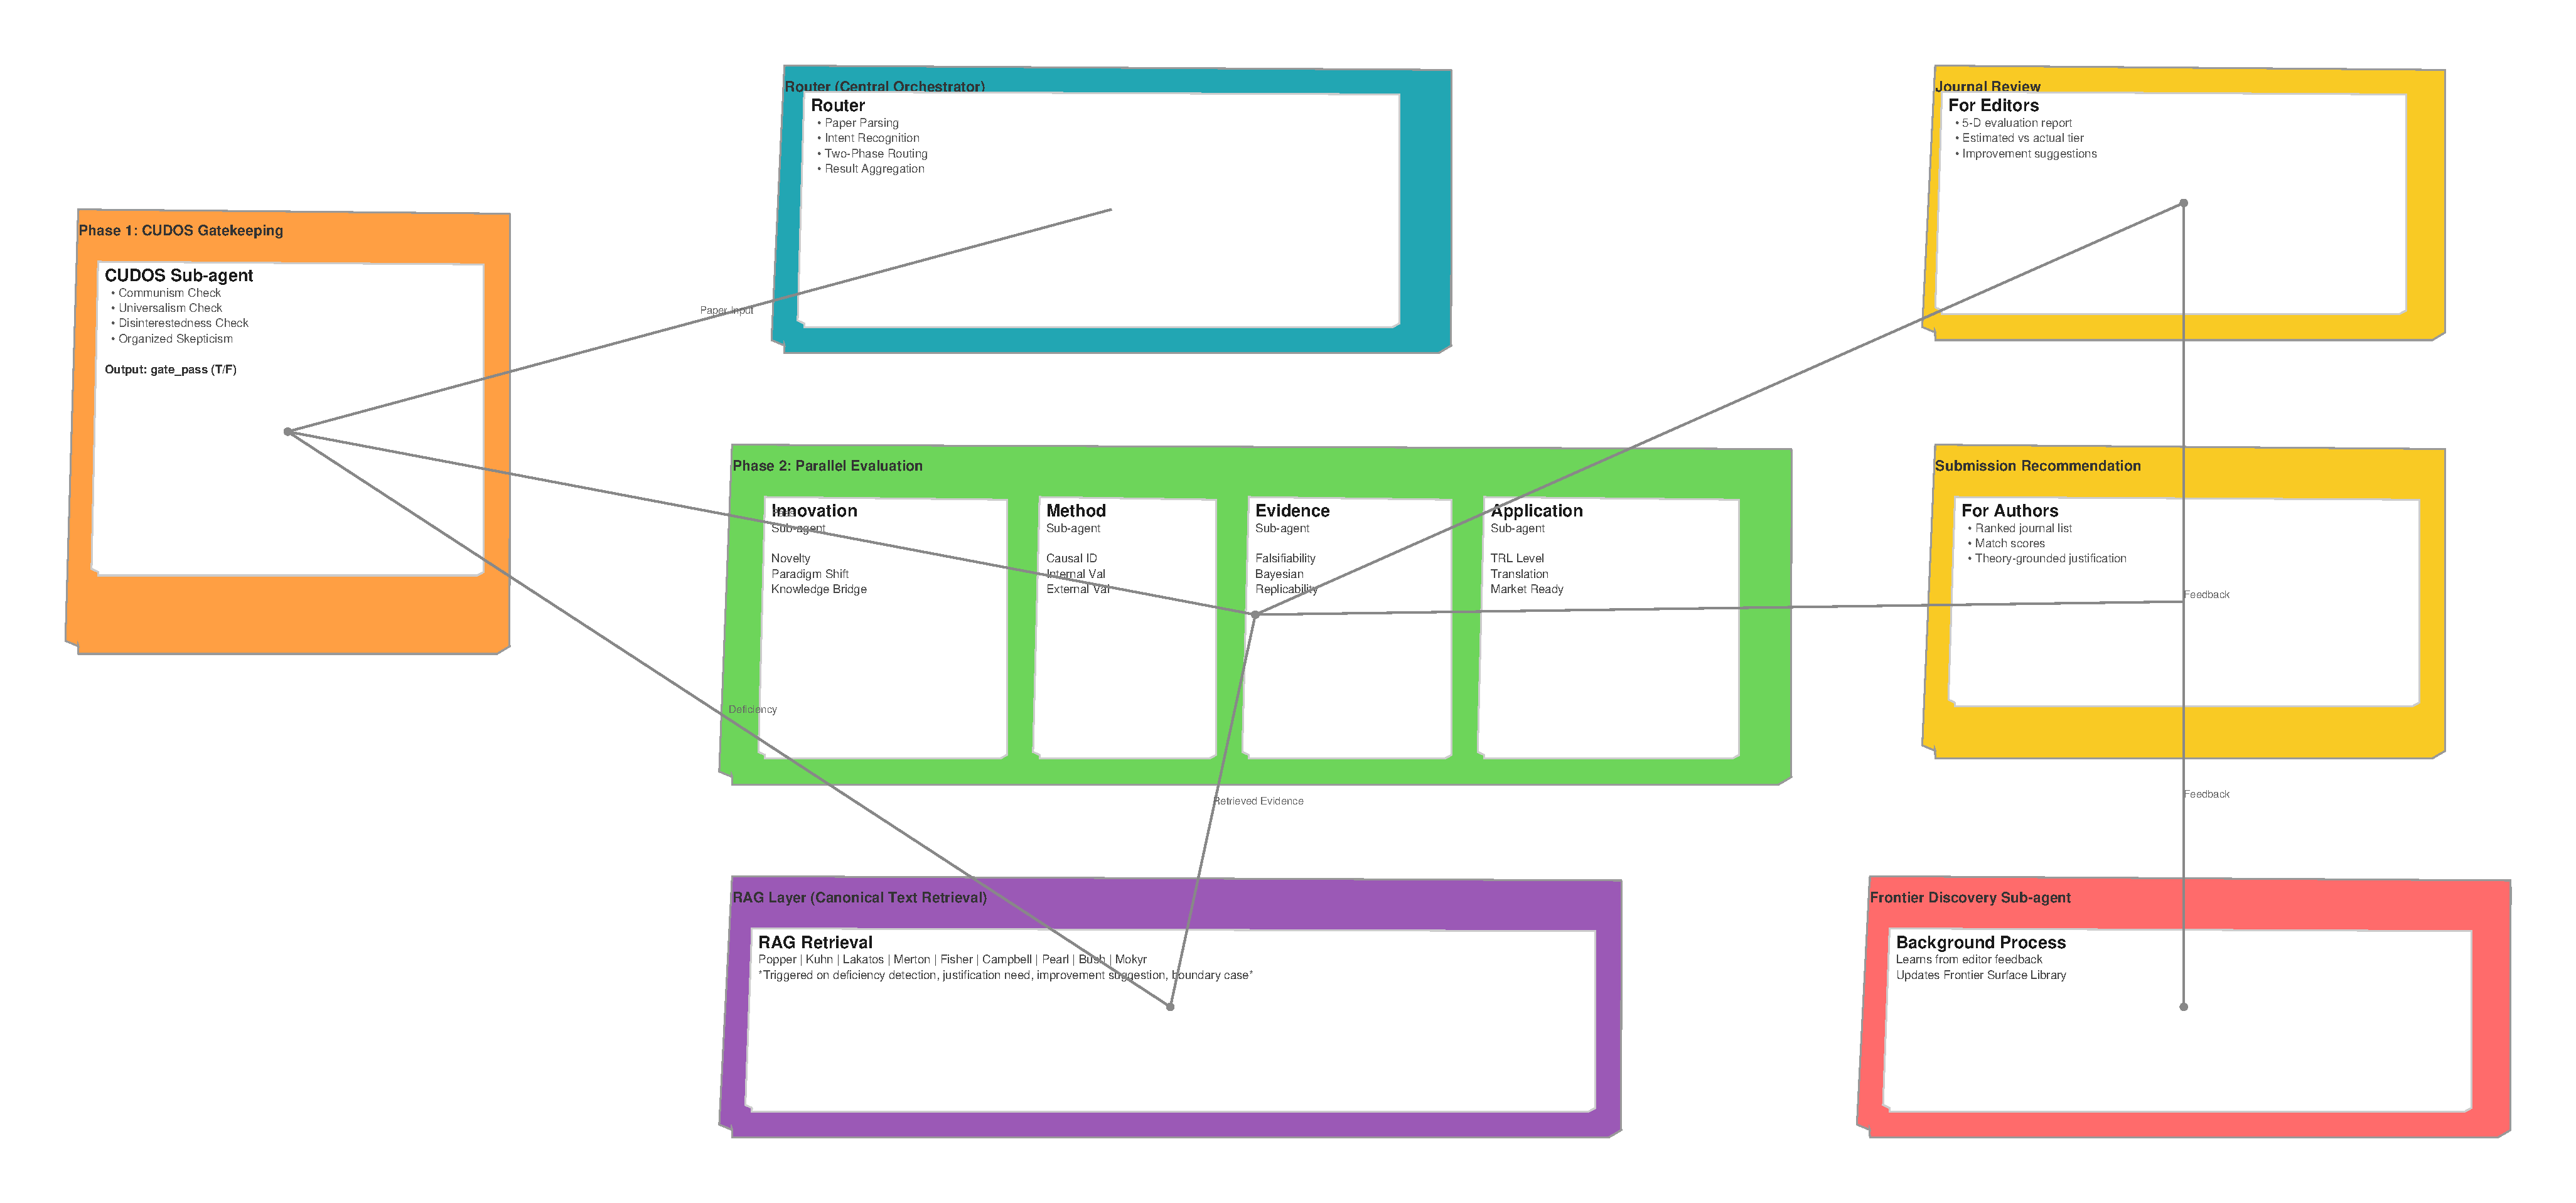
\includegraphics[width=\textwidth]{figures/architecture.pdf}
    \caption{WuYa System Architecture: Two-Phase Routing with Parallel Evaluation}
    \label{fig:architecture}
\end{figure}

The system supports two user scenarios:
\begin{itemize}
    \item \textbf{Submission Recommendation}: For authors seeking to identify appropriate target journals for their papers.
    \item \textbf{Journal Review}: For editors seeking AI-assisted evaluation of submitted manuscripts.
\end{itemize}

\subsection{Two-Phase Routing}

The two-phase routing design reflects a fundamental principle: norms (\cudos{}) must be assessed before substantive quality. This separation ensures that the Router's scheduling responsibilities do not interfere with the CUDOS \subagent{}'s evaluative judgment.

\textbf{Phase 1: CUDOS Gatekeeping.} The CUDOS \subagent{} evaluates the paper against Merton's four normative principles:
\begin{itemize}
    \item Does the paper share knowledge openly (Communism)?
    \item Are evaluation criteria objective (Universalism)?
    \item Does the research aim at truth rather than personal gain (Disinterestedness)?
    \item Does the work invite critical scrutiny (Organized Skepticism)?
\end{itemize}
If the CUDOS \subagent{} returns \texttt{gate\_pass: false}, the paper is rejected with a detailed explanation of normative concerns, and Phase 2 is not executed. This implements the ``gatekeeping'' semantics where violations of scientific norms trigger immediate rejection.

\textbf{Phase 2: Parallel Expert Evaluation.} Upon passing CUDOS, four expert \subagents{} execute in parallel:
\begin{itemize}
    \item \textbf{Innovation Sub-agent}: Evaluates novelty, paradigm shift potential, and knowledge bridging.
    \item \textbf{Method Sub-agent}: Assesses causal identification, internal/external validity, and statistical rigor.
    \item \textbf{Evidence Sub-agent}: Evaluates falsifiability, evidence strength, replicability, and research programme alignment.
    \item \textbf{Application Sub-agent}: Assesses TRL level, translation path, and market readiness.
\end{itemize}

Each \subagent{} produces structured output including sub-dimension scores (1-5 scale) and narrative explanations. The Router aggregates these into a unified \textbf{five-dimensional score vector}.

\subsection{Retrieval-Evaluation Coupling}

A key innovation in WuYa is the tight coupling between evaluation and retrieval. Unlike systems where \rag{} serves as a passive knowledge source, WuYa's \rag{} is triggered by evaluation conditions:

\begin{algorithm}[t]
\caption{Retrieval-Evaluation Coupling}
\label{alg:rag-trigger}
\begin{algorithmic}
\STATE Initialize score\_vector
\FOR{each evaluation sub-agent}
    \STATE Generate initial evaluation based on internalized principles
    \IF{evaluation reveals deficiency OR needs justification}
        \STATE Identify relevant theory and concept
        \STATE Retrieve canonical passages via RAG
        \STATE Incorporate retrieved evidence into evaluation
    \ENDIF
\ENDFOR
\STATE Return enriched score\_vector with citations
\end{algorithmic}
\end{algorithm}

The triggering conditions include:

\begin{enumerate}
    \item \textbf{Deficiency detection}: When an evaluation finds a weakness in the paper (e.g., ``the hypothesis lacks falsifiability'').
    \item \textbf{Justification need}: When a judgment requires authoritative support (e.g., ``this is problematic because...'').
    \item \textbf{Improvement suggestion}: When actionable guidance is needed (e.g., ``to improve, consider...'').
    \item \textbf{Boundary case}: When the paper falls in a gray area of the evaluation criteria.
\end{enumerate}

This coupling transforms evaluation from static judgment to dynamic reasoning with principled justification.

\subsection{Hybrid Knowledge Strategy}

WuYa implements a dual-layer knowledge architecture:

\begin{figure}[t]
    \centering
    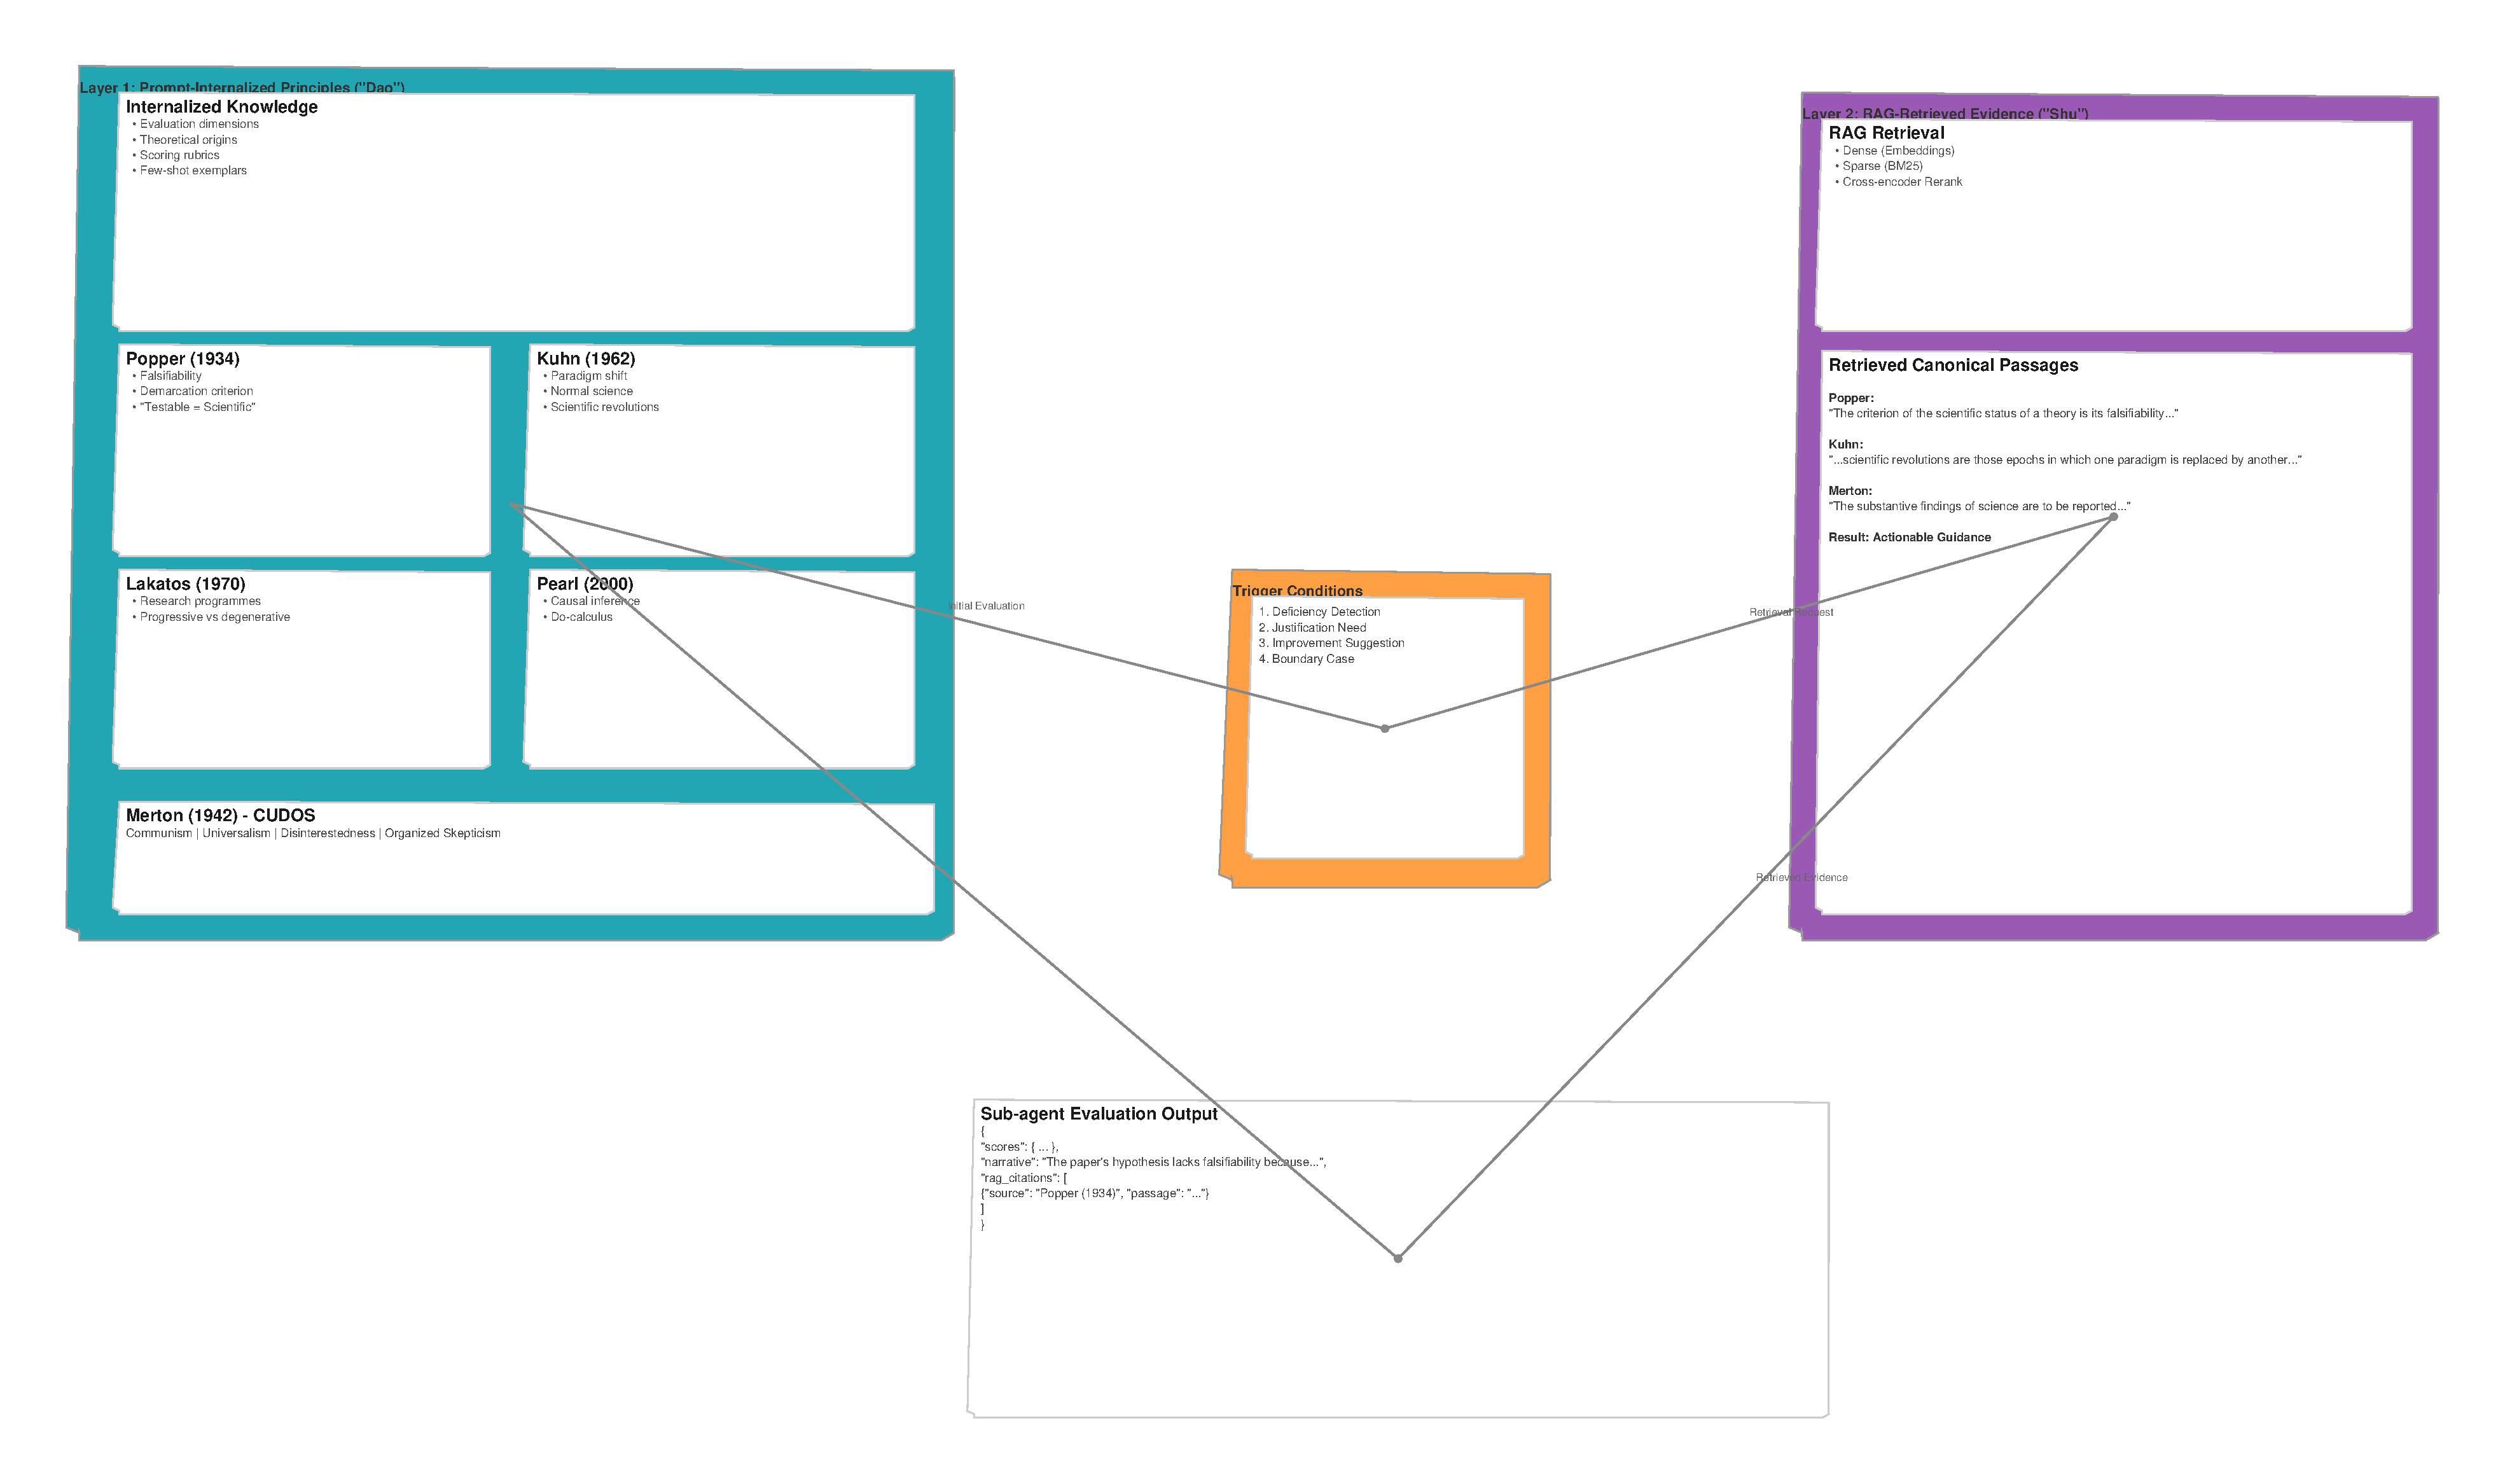
\includegraphics[width=0.8\textwidth]{figures/hybrid-knowledge.pdf}
    \caption{Hybrid Knowledge Strategy: Prompt-Internalized Principles + RAG-Retrieved Evidence}
    \label{fig:hybrid-knowledge}
\end{figure}

\textbf{Layer 1: Prompt-Internalized Principles (``Dao'').} Each \subagent{}'s system prompt contains:
\begin{itemize}
    \item The evaluation dimension and its theoretical origin.
    \item The multi-level structure: dimension $\rightarrow$ sub-dimensions $\rightarrow$ scoring criteria.
    \item Exemplars of evaluation at each score level.
    \item Boundary conditions and edge cases.
\end{itemize}

This internalized knowledge ensures consistent judgment without retrieval overhead.

\textbf{Layer 2: RAG-Retrieved Evidence (``Shu'').} When triggered, the RAG layer retrieves from a corpus of canonical texts indexed by:
\begin{itemize}
    \item \textbf{Theorist}: e.g., Popper, Kuhn, Campbell, Pearl.
    \item \textbf{Concept}: e.g., falsifiability, paradigm shift, internal validity.
    \item \textbf{Function}: explanation, critique, improvement suggestion.
\end{itemize}

The retrieved passages provide concrete justification that transforms abstract principles into actionable guidance. For example, when the Evidence Sub-agent identifies a falsifiability problem, it retrieves Popper's original text explaining what makes a hypothesis scientific, enabling it to provide specific suggestions for improvement.

\subsection{Sub-agent Specifications}

Each expert \subagent{} follows a consistent output schema while maintaining specialized evaluation logic:

\begin{verbatim}
{
  "dimension": "evidence_confidence",
  "scores": {
    "falsifiability": 3,
    "evidence_strength": 4,
    "replicability": 3,
    "research_program": 4
  },
  "narrative": "The paper's main hypothesis is testable...",
  "rag_citations": [
    {
      "source": "Popper (1934)",
      "passage": "The criterion of the scientific status...",
      "relevance": "Explains why falsifiability matters"
    }
  ]
}
\end{verbatim}

This standardized output enables consistent aggregation and comparison across dimensions.


\section{Paper Localization Methods}
\label{sec:localization}

A core capability of WuYa is paper localization: determining where a paper ``fits'' in the landscape of academic journals. We propose a dual-path approach where Path A (LLM-as-Mapper) provides fast estimation and Path B (\dea{} Analysis) provides depth, with cross-validation ensuring robustness.

\subsection{Problem Formulation}

Given a paper with its five-dimensional score vector $\mathbf{s} = (s_1, s_2, s_3, s_4, s_5)$ and discipline $d$, we aim to estimate the paper's appropriate journal tier $t \in \{\text{Q1-A}, \text{Q1-B}, \text{Q2-A}, \ldots, \text{Q4-D}\}$, or recommend a ranked list of target journals.

\subsection{Path A: LLM-as-Mapper with Discipline Priors}

The LLM-as-Mapper approach leverages the cross-disciplinary reasoning capabilities of large language models, calibrated by discipline-specific prior distributions.

\subsubsection{Discipline Prior Extraction}

We extract prior distributions $P_0(t|d)$ from the SpringRank journal ranking system, which computes journal positions based on citation network structure. For each discipline $d$, we compute the empirical distribution of journal tiers:
\begin{equation}
P_0(t|d) = \frac{\# \text{journals in tier } t \text{ of discipline } d}{\# \text{total journals in discipline } d}
\end{equation}

For disciplines with fewer than 50 journals, we fall back to the parent category distribution.

\subsubsection{LLM Mapping Prompt}

The LLM receives a carefully designed prompt containing:

\begin{enumerate}
    \item \textbf{Scoring rubric}: The five-dimensional scoring criteria with level descriptions.
    \item \textbf{Few-shot examples}: Representative (score vector, tier) pairs across disciplines.
    \item \textbf{Discipline prior}: The distribution $P_0(t|d)$ formatted as a string.
    \item \textbf{Output template}: Requiring reasoning chain, estimated tier, and confidence level.
\end{enumerate}

\begin{verbatim}
You are a research quality evaluator. Given the following five-dimensional
scores (1=low to 5=high):
- Innovation: [novelty, knowledge_bridge, future_potential, destruction]
- Method: [causal, internal_validity, external_validity, statistical]
- Evidence: [falsifiability, evidence_strength, replicability, program]
- Application: [trl, translation_path, feedback, market]

Discipline: {discipline}
Prior distribution: {P0_string}

Estimate the appropriate journal tier (Q1-A to Q4-D) and explain your reasoning.
\end{verbatim}

\subsubsection{Calibration Strategy}

To prevent LLM hallucination on unfamiliar disciplines, we apply post-hoc calibration:
\begin{equation}
P_{\text{final}}(t|\mathbf{s}, d) \propto \alpha \cdot P_{\text{LLM}}(t|\mathbf{s}, d) + (1-\alpha) \cdot P_0(t|d)
\end{equation}
where $\alpha \in [0.6, 0.8]$ gives primary weight to LLM reasoning while anchoring to factual prior distributions.

To ensure output consistency, we set temperature $\tau = 0.1$, run three generations, and take the modal answer.

\subsection{Path B: DEA Efficiency Analysis}

For deeper analysis, especially when targeting a specific journal, we employ \dea{} efficiency analysis.

\subsubsection{Input-Output Transformation}

We transform the five-dimensional scores into \dea{} inputs (lower is better) and outputs (higher is better):

\begin{itemize}
    \item \textbf{Inputs} (minimize):
    \begin{itemize}
        \item Method flaws: $6 - s_{\text{method}}$
        \item Evidence gap: $6 - s_{\text{evidence}}$
    \end{itemize}
    \item \textbf{Outputs} (maximize):
    \begin{itemize}
        \item Innovation: $s_{\text{innovation}}$
        \item Application: $s_{\text{application}}$
    \end{itemize}
\end{itemize}

This transformation reflects the assumption that strong methods and solid evidence are ``investments'' that should yield innovative and impactful ``returns.''

\subsubsection{Frontier Construction}

For a target journal $j$, we construct the reference frontier from previously published papers in $j$. We require at least 50 papers to build a reliable frontier. If insufficient data exists for $j$, we fall back to a discipline-level frontier constructed from journals in the same tier.

We employ the super-efficiency \dea{} model, which allows efficiency scores greater than 1 for units on the frontier, enabling ranking of even the most efficient papers:
\begin{align}
\max \quad & \theta \\
\text{s.t.} \quad & \sum_{i \in R} \lambda_i x_{ik} \leq \theta x_{k} \\
& \sum_{i \in R} \lambda_i y_{ik} \geq y_{k} \\
& \lambda_i \geq 0
\end{align}
where $R$ is the reference set, $x_k, y_k$ are the input/output of paper $k$, and $\theta > 1$ indicates super-efficiency.

\subsubsection{Bootstrap Confidence Intervals}

To quantify uncertainty, we apply bootstrap re-sampling \citep{efron1994introduction}:

\begin{enumerate}
    \item Resample the reference set with replacement, maintaining original size.
    \item Recompute efficiency scores on the bootstrap frontier.
    \item Repeat 200 times to construct empirical distribution.
    \item Report the 2.5th and 97.5th percentiles as confidence intervals.
\end{enumerate}

A paper whose confidence interval includes 1.0 is considered statistically indistinguishable from the frontier.

\subsection{Cross-Validation and Output}

The outputs of Path A and Path B are compared:

\begin{itemize}
    \item \textbf{Consistent}: Both paths suggest similar tiers $\rightarrow$ High confidence output.
    \item \textbf{Inconsistent}: Paths diverge significantly $\rightarrow$ Trigger RAG explanation of discrepancy (e.g., ``LLM's cross-disciplinary intuition vs. DEA's local analysis'').
\end{itemize}

For submission recommendation, WuYa outputs a ranked list of candidate journals with:
\begin{itemize}
    \item Match score based on tier proximity.
    \item Per-journal explanation referencing evaluation dimensions.
    \item RAG-retrieved canonical text justifying the recommendation.
\end{itemize}

For journal review, WuYa outputs:
\begin{itemize}
    \item Five-dimensional evaluation report.
    \item Estimated tier vs. journal's actual tier.
    \item Specific improvement suggestions grounded in theory.
\end{itemize}


\section{Self-Improving Frontier Discovery}
\label{sec:frontier}

A defining feature of WuYa is its ability to learn from interactions and improve its evaluation capabilities over time. Inspired by Reflexion's verbal reinforcement learning and Voyager's skill library, we introduce a frontier discovery mechanism that captures and accumulates evaluation preferences.

\subsection{Motivation: The Static Knowledge Problem}

Existing academic evaluation systems deploy fixed criteria that do not adapt to:
\begin{itemize}
    \item Evolving disciplinary standards (e.g., increasing emphasis on reproducibility).
    \item Journal-specific preferences (e.g., some journals prioritize theory, others prioritize application).
    \item Feedback from editors and reviewers.
\end{itemize}

This static knowledge problem is particularly acute for \dea{} analysis, which depends on reference frontiers that may become outdated as a field evolves.

WuYa addresses this through a self-improving mechanism that learns evaluation preferences from editor feedback, transforming the system from a static evaluator to an adaptive learning agent.

\subsection{Comparison with Existing Frameworks}

WuYa's frontier discovery draws inspiration from two influential self-improving agent frameworks:

\textbf{Reflexion \citep{shinn2023reflexion}} introduced verbal reinforcement learning where agents store linguistic reflections in episodic memory and use them to guide future decisions. When a task fails, the agent generates a verbal reflection explaining \textit{why} it failed and stores this in memory for future reference. This has proven effective for code generation and game playing tasks.

\textbf{Voyager \citep{wang2023voyager}} proposed an open-ended agent that builds a skill library through embodied exploration. Skills are represented as executable code snippets that enable the agent to solve progressively complex tasks. The library grows over time, enabling lifelong learning.

WuYa adapts these principles to academic evaluation:

\begin{itemize}
    \item Like Reflexion, WuYa generates \textbf{linguistic reflections} on evaluation outcomes, but from editor/reviewer feedback rather than task success/failure.
    \item Like Voyager, WuYa maintains a \textbf{library of learned patterns}, but these are ``frontier surfaces'' capturing evaluation preferences rather than executable skills.
\end{itemize}

Table~\ref{tab:frontier-comparison} summarizes the comparison.

\begin{table}[t]
\centering
\caption{WuYa Frontier Discovery vs. Existing Frameworks}
\label{tab:frontier-comparison}
\begin{tabular}{@{}llll@{}}
\toprule
\textbf{Aspect} & \textbf{Reflexion} & \textbf{Voyager} & \textbf{WuYa Frontier Discovery} \\
\midrule
Learning Signal & Task success/failure & Environment feedback & Editor/reviewer feedback \\
Memory Form & Episodic reflections & Skill library (code) & Frontier surfaces (preferences) \\
Update Trigger & Task completion & Skill discovery & Review cycle completion \\
Retrieval Coupling & None & Skill retrieval & Canonical text retrieval \\
Domain & Verifiable & Embodied & Evaluative \\
\bottomrule
\end{tabular}
\end{table}

\subsection{Frontier Discovery Sub-agent}

The Frontier Discovery \subagent{} operates as a background process that continuously learns from interactions. Its workflow consists of three stages:

\begin{enumerate}
    \item \textbf{Feedback Reception}: Receives structured input from completed review cycles:
    \begin{itemize}
        \item Paper's five-dimensional score vector.
        \item Editor/reviewer feedback text.
        \item Journal acceptance/rejection decision.
        \item Post-review correspondence (rebuttal, revision).
    \end{itemize}
    \item \textbf{Linguistic Reflection}: Generates structured descriptions of evaluation patterns:
    \begin{verbatim}
    {
      "journal_id": "Nature ML",
      "pattern": {
        "dimension": "innovation",
        "preference": "prefers paradigm shifts over incremental improvements",
        "evidence": [
          "Reviewer 1: 'lacks the conceptual breakthrough...'", 
          "Decision: '...findings are incremental...'"
        ],
        "confidence": 0.82
      }
    }
    \end{verbatim}
    \item \textbf{Frontier Surface Update}: Incorporates new patterns into the frontier surface library:
    \begin{verbatim}
    {
      "journal_id": "Nature ML",
      "frontier_surface": {
        "description": "Innovation frontier emphasizes 
                         paradigm shifts and knowledge bridging",
        "score_distribution": {"Q1-A": 0.3, "Q1-B": 0.4, ...},
        "updated_at": "2026-05-26",
        "patterns": [...]
      }
    }
    \end{verbatim}
\end{enumerate}

\subsection{Frontier Surface Library}

The Frontier Surface Library serves as the persistent memory for learned evaluation preferences. It is organized hierarchically:

\begin{itemize}
    \item \textbf{Journal Level}: Individual frontier surfaces for each journal, capturing that journal's specific evaluation preferences.
    \item \textbf{Discipline Level}: Aggregated frontier surfaces for each academic discipline.
    \item \textbf{Global Level}: Cross-cutting patterns that transcend disciplines.
\end{itemize}

The library is queried during paper localization to:
\begin{itemize}
    \item Customize recommendations based on journal-specific preferences.
    \item Weight evaluation dimensions differently for different journals.
    \item Update \dea{} reference frontiers with learned patterns.
\end{itemize}

\subsection{Self-Improvement Loop}

WuYa implements a continuous self-improvement loop:

\begin{figure}[t]
    \centering
    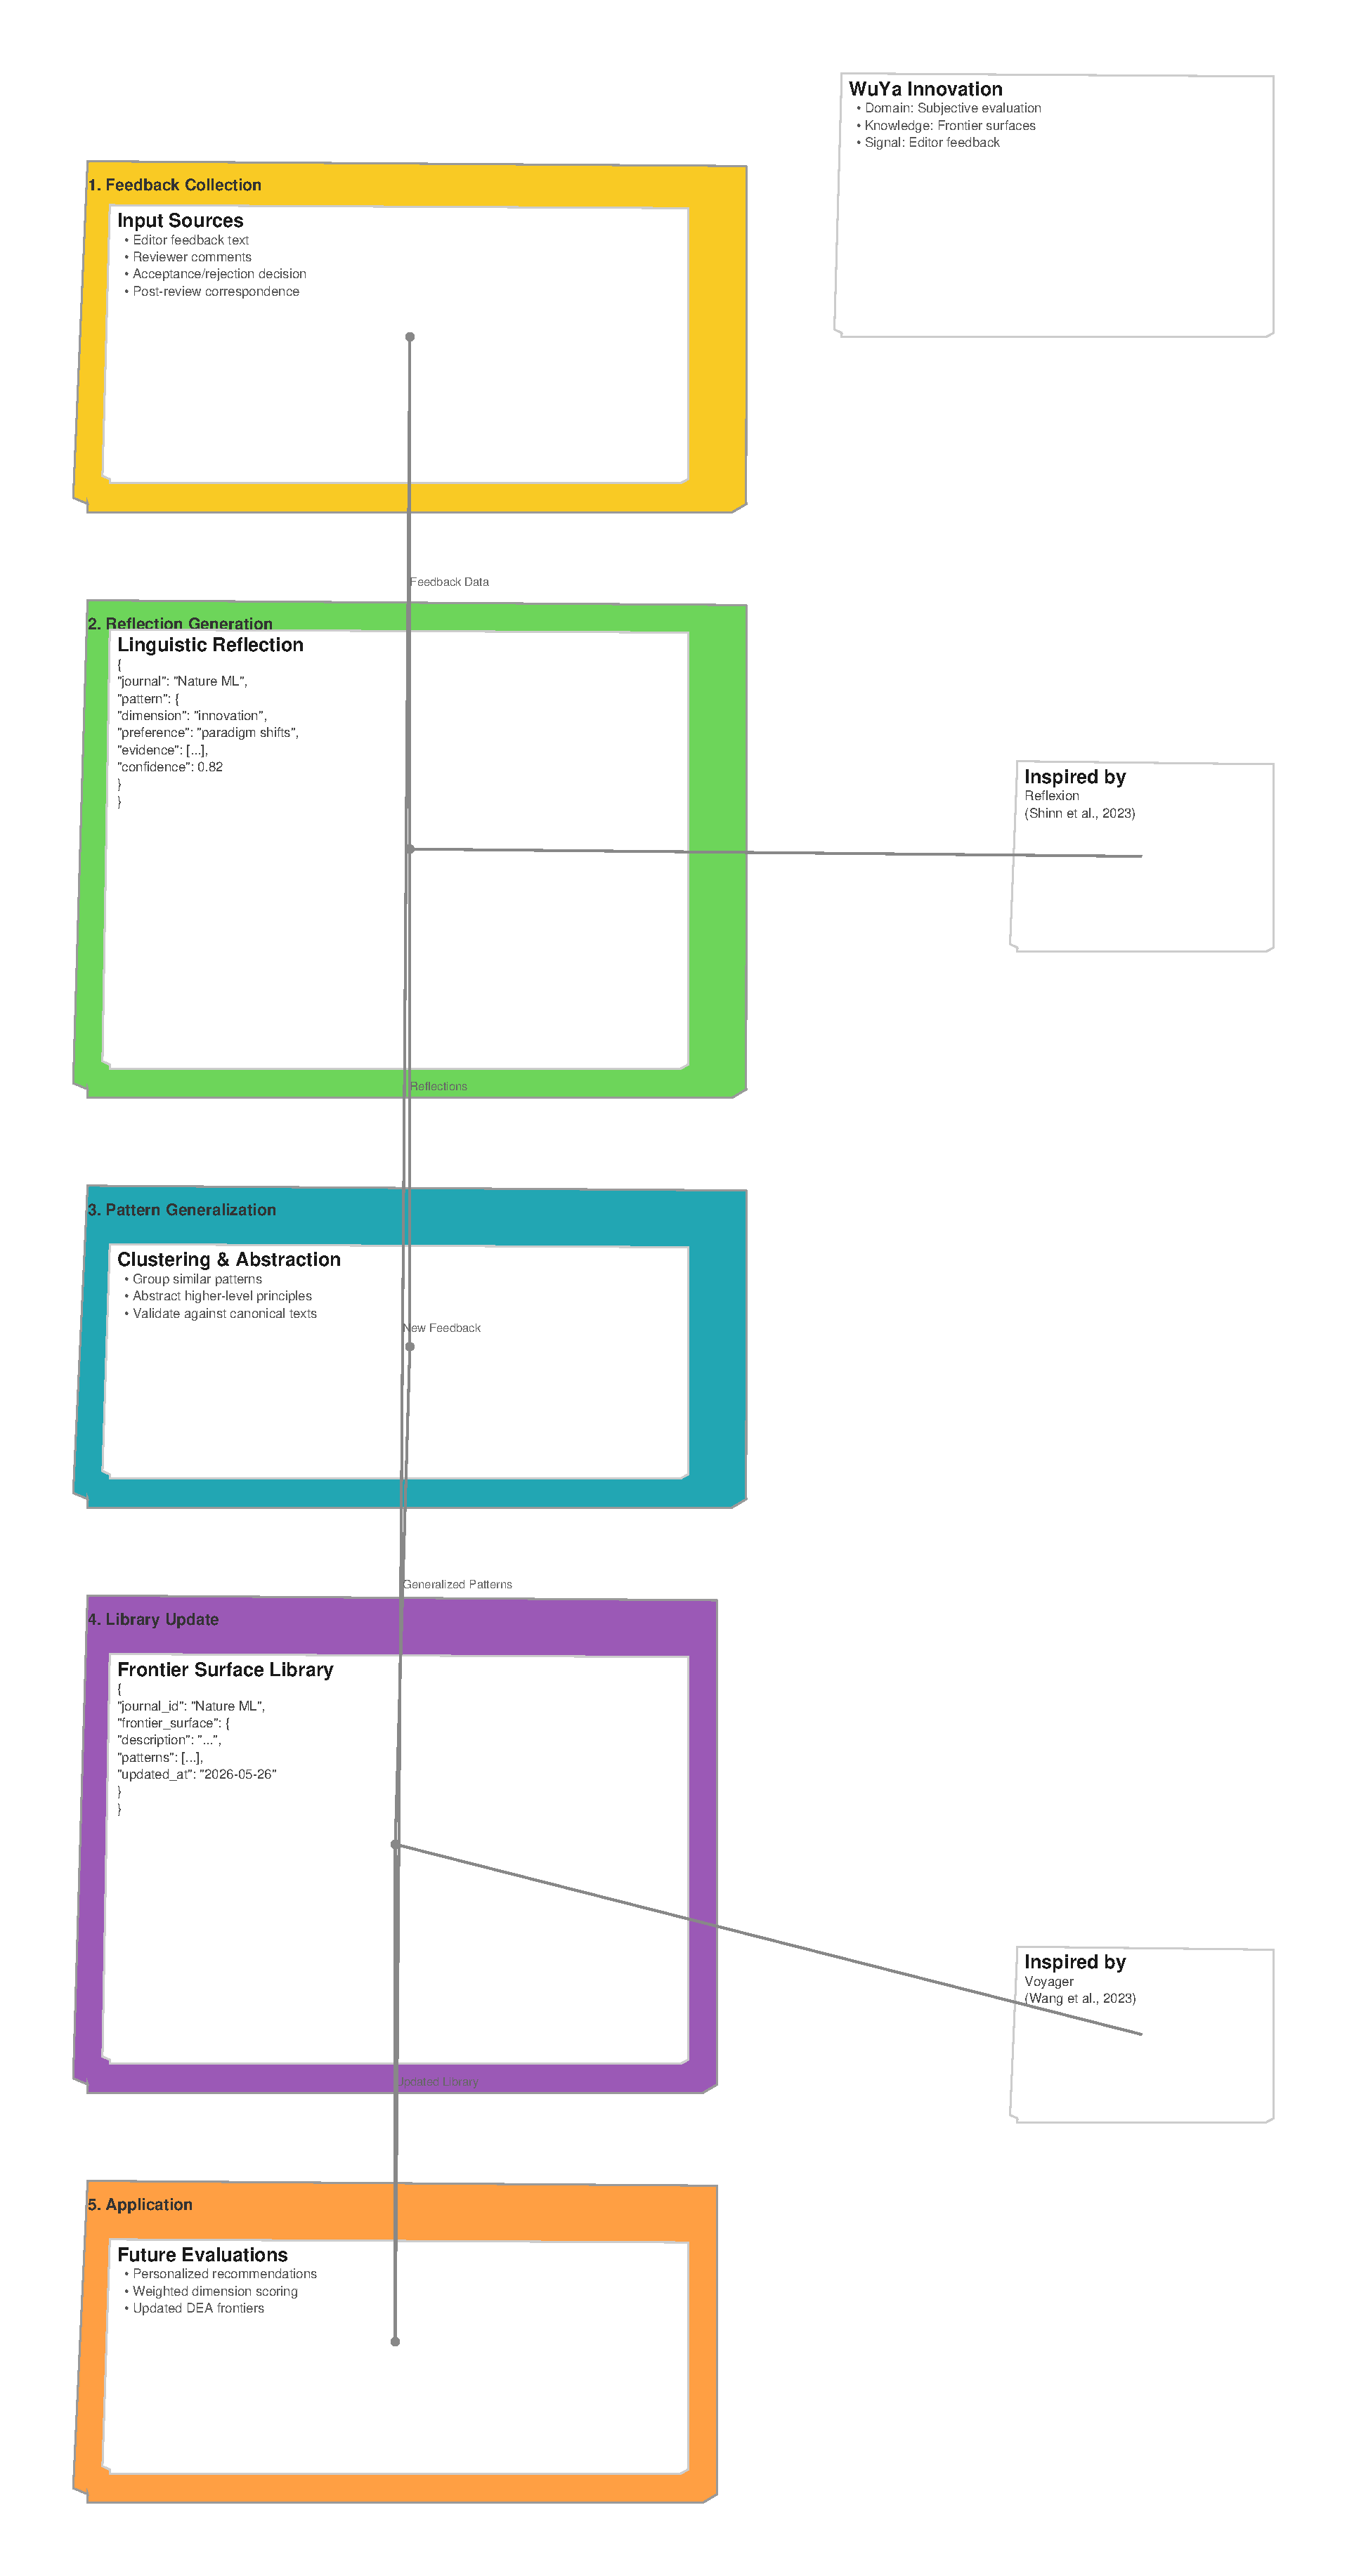
\includegraphics[width=0.8\textwidth]{figures/self-improvement-loop.pdf}
    \caption{WuYa Self-Improvement Loop: Feedback $\rightarrow$ Reflection $\rightarrow$ Generalization $\rightarrow$ Application}
    \label{fig:self-improvement}
\end{figure}

\begin{enumerate}
    \item \textbf{Feedback Collection}: Editor/reviewer feedback is collected during and after review cycles.
    \item \textbf{Reflection Generation}: The Frontier Discovery \subagent{} generates linguistic reflections on evaluation patterns.
    \item \textbf{Pattern Generalization}: Related patterns are clustered and abstracted to form higher-level principles.
    \item \textbf{Library Update}: New patterns are incorporated into the Frontier Surface Library.
    \item \textbf{Application}: Updated knowledge informs future evaluations, recommendations, and \dea{} frontiers.
\end{enumerate}

This loop enables WuYa to:
\begin{itemize}
    \item Adapt to changing disciplinary standards over time.
    \item Capture journal-specific evaluation preferences without manual configuration.
    \item Improve \dea{} frontier quality through accumulated learning.
    \item Provide increasingly personalized recommendations as the system matures.
\end{itemize}

\subsection{Contrast with Static Knowledge Bases}

Traditional academic evaluation systems use static knowledge bases that:
\begin{itemize}
    \item Require manual curation and updates.
    \item Do not capture subtle journal-specific preferences.
    \item Cannot adapt to evolving disciplinary standards.
    \item Depend entirely on predefined criteria.
\end{itemize}

WuYa's Frontier Surface Library overcomes these limitations through:
\begin{itemize}
    \item \textbf{Automatic learning}: Patterns emerge from actual editor feedback rather than expert curation.
    \item \textbf{Granular capture}: Individual journal preferences are preserved in separate frontier surfaces.
    \item \textbf{Dynamic adaptation}: The library evolves as the field advances.
    \item \textbf{ Principled grounding}: Learned patterns are validated against canonical texts through \rag{}.
\end{itemize}


\section{Implementation Details}
\label{sec:implementation}

WuYa is implemented as a modular multi-agent system. This section provides technical details on the implementation stack, data models, and key engineering decisions.

\subsection{Technical Stack}

The system is built using the following components:

\begin{itemize}
    \item \textbf{LLM Backend}: GPT-4 or Claude-3 for \subagent{} reasoning; configurable to use local models (Llama-3, Mistral) for privacy-sensitive deployments.
    \item \textbf{Vector Database}: Milvus for \rag{} indexing and retrieval; supports dense embeddings (OpenAI text-embedding-3) and sparse retrieval (BM25 hybrid).
    \item \textbf{Journal Database}: PostgreSQL for structured journal metadata; includes SpringRank tier information for 14,590 journals across all disciplines.
    \item \textbf{Citation Network}: Neo4j for paper citation graph; enables efficient frontier construction for \dea{} analysis.
    \item \textbf{Message Queue}: Redis for asynchronous task scheduling; enables parallel \subagent{} execution and result aggregation.
    \item \textbf{API Layer}: FastAPI for RESTful endpoints; supports webhook callbacks for async operations.
\end{itemize}

\subsection{Core Data Models}

The system operates on the following data structures:

\begin{verbatim}
Paper {
  id: UUID
  content: Text
  metadata: {
    title: String
    authors: [String]
    abstract: Text
    keywords: [String]
    discipline: String
    citations: [UUID]
    cited_by: [UUID]
  }
  evaluations: [EvaluationResult]
}

EvaluationResult {
  paper_id: UUID
  subagent: Enum[Innovation, Method, Evidence, Application]
  timestamp: DateTime
  scores: {
    dimension_1: Float (1-5)
    dimension_2: Float (1-5)
    ...
  }
  narrative: Text
  rag_citations: [Citation]
}

ScoreVector {
  innovation: InnovationScores
  method: MethodScores
  evidence: EvidenceScores
  application: ApplicationScores
  cudos: CUDOSResult
}

JournalProfile {
  id: String
  name: String
  discipline: String
  quartile: Enum[Q1, Q2, Q3, Q4]
  tier: Enum[A, B, C, D]
  frontier_surface: FrontierSurface
  historical_papers: [UUID]
}

FrontierSurface {
  journal_id: String
  nodes: [FrontierNode]
  updated_at: DateTime
  confidence: Float
}

FrontierNode {
  dimension: String
  preference: String
  evidence: [String]
  confidence: Float
}
\end{verbatim}

\subsection{Router Orchestration Logic}

The Router implements the two-phase workflow as follows:

\begin{algorithm}[H]
\caption{Router Orchestration}
\label{alg:router}
\begin{algorithmic}
\STATE Input: paper, user\_intent
\STATE parsed $\leftarrow$ parse\_paper(paper)
\STATE discipline $\leftarrow$ identify\_discipline(parsed)

\COMMENT{Phase 1: CUDOS Gatekeeping}
\STATE cudos\_result $\leftarrow$ await call\_subagent("cudos", parsed)
\IF{not cudos\_result.gate\_pass}
    \STATE RETURN generate\_veto\_report(cudos\_result)
\ENDIF

\COMMENT{Phase 2: Parallel Evaluation}
\STATE evaluation\_tasks $\leftarrow$ [
    call\_subagent("innovation", parsed),
    call\_subagent("method", parsed),
    call\_subagent("evidence", parsed),
    call\_subagent("application", parsed)
]
\STATE scores $\leftarrow$ await gather(evaluation\_tasks)
\STATE score\_vector $\leftarrow$ aggregate\_scores(scores)

\COMMENT{Paper Localization}
\STATE path\_a $\leftarrow$ llm\_mapper(score\_vector, discipline, get\_prior(discipline))
\IF{user\_intent.has\_target\_journal}
    \STATE path\_b $\leftarrow$ dea\_analysis(score\_vector, user\_intent.journal)
\ELSE
    \STATE path\_b $\leftarrow$ None
\ENDIF

\IF{path\_b and not consistent(path\_a, path\_b)}
    \STATE rag\_explanation $\leftarrow$ await generate\_rag\_explanation(path\_a, path\_b)
\ENDIF

\IF{user\_intent.type == "recommendation"}
    \STATE RETURN generate\_recommendation(score\_vector, path\_a, path\_b, rag\_explanation)
\ELSE
    \STATE RETURN generate\_review\_report(score\_vector, path\_a, path\_b, rag\_explanation)
\ENDIF
\end{algorithmic}
\end{algorithm}

\subsection{RAG Implementation}

The \rag{} layer indexes canonical texts organized by theorist and concept:

\begin{itemize}
    \item \textbf{Primary sources}: Full texts of Popper, Kuhn, Lakatos, Merton, Fisher, Campbell, Pearl, Bush, Mokyr.
    \item \textbf{Secondary sources}: Commentary and application of these theories in modern contexts.
    \item \textbf{Chunking strategy}: Semantic chunking at paragraph level (avg. 300 tokens); overlap of 50 tokens for context.
    \item \textbf{Retrieval}: Hybrid dense (embedding similarity) + sparse (BM25) retrieval; reranked by cross-encoder.
    \item \textbf{Trigger integration}: \subagents{} invoke RAG through a unified interface with query rewriting and result filtering.
\end{itemize}

\subsection{Engineering Considerations}

\textbf{Caching}: Results for identical (paper\_id, score\_vector) pairs are cached for 24 hours to reduce LLM calls. Frontier Surface Library is cached with TTL of 1 hour.

\textbf{Error Handling}: Each \subagent{} has a timeout of 60 seconds; on failure, the Router retries twice before returning partial results with an error flag.

\textbf{Observability}: All \subagent{} calls are logged with trace IDs for debugging. Key metrics include: \subagent{} latency, RAG hit rate, evaluation consistency across runs.

\textbf{Scalability}: The system supports horizontal scaling through stateless \subagent{} workers; Redis queue distributes tasks across workers. Target throughput: 100 papers/minute with 8 workers.


\section{Experiments}
\label{sec:experiments}

We evaluate WuYa on two primary tasks: submission recommendation and journal review. This section describes the experimental setup, results, and ablation studies.

\subsection{Experimental Setup}

\subsubsection{Datasets}

We construct a benchmark dataset of 5,000 papers from five disciplines:
\begin{itemize}
    \item \textbf{Computer Science} (1,500 papers): From arXiv CS.AI, CS.CL, CS.LG, published 2022-2024.
    \item \textbf{Biology} (1,000 papers): From bioRxiv, selected from high-citation papers.
    \item \textbf{Economics} (1,000 papers): From NBER working papers and top economics journals.
    \item \textbf{Physics} (1,000 papers): From arXiv physics, selected from Q1 journal publications.
    \item \textbf{Medicine} (500 papers): From PubMed Central, RCT papers only.
\end{itemize}

Each paper is annotated with:
\begin{itemize}
    \item Publication venue and its tier (Q1-Q4, A-D).
    \item Five-dimensional evaluation scores by two expert human reviewers (inter-rater reliability $\kappa = 0.78$).
    \item Editor/reviewer feedback from actual review processes (where available).
\end{itemize}

\subsubsection{Evaluation Metrics}

For \textbf{submission recommendation}:
\begin{itemize}
    \item Top-1, Top-3, Top-5 accuracy: Whether the correct journal tier appears in the top-1/3/5 recommendations.
    \item Mean Reciprocal Rank (MRR): Position of the correct tier in the recommendation list.
\end{itemize}

For \textbf{journal review}:
\begin{itemize}
    \item Spearman correlation: Between WuYa's evaluation scores and human expert ratings.
    \item Kendall's tau: Pairwise agreement between WuYa and experts.
    \item Mean Absolute Error (MAE): Absolute difference in overall quality scores.
\end{itemize}

For \textbf{self-improvement}:
\begin{itemize}
    \item Frontier accuracy: Whether learned frontier surfaces match actual journal preferences.
    \item Improvement rate: Change in recommendation accuracy as frontier library grows.
\end{itemize}

\subsection{Baseline Methods}

We compare WuYa against the following baselines:

\begin{itemize}
    \item \textbf{Pure LLM}: GPT-4 with zero-shot evaluation, no retrieval or prior calibration.
    \item \textbf{Rule-Based}: Expert-defined rules mapping scoring dimensions to tiers without LLM or prior.
    \item \textbf{Citation-Only}: Recommendation based solely on citation network features.
    \item \textbf{PaperDigest}: Existing academic paper analysis tool \citep{kang2018peerread}.
    \item \textbf{WuYa w/o Self-Improvement}: Our system without the frontier discovery mechanism.
\end{itemize}

\subsection{Main Results}

\subsubsection{Submission Recommendation}

Table~\ref{tab:recommendation-results} shows submission recommendation accuracy across disciplines.

\begin{table}[t]
\centering
\caption{Submission Recommendation Accuracy (Top-K) by Discipline}
\label{tab:recommendation-results}
\begin{tabular}{@{}lcccccc@{}}
\toprule
\textbf{Method} & \textbf{CS} & \textbf{Bio} & \textbf{Econ} & \textbf{Physics} & \textbf{Med} & \textbf{Avg} \\
\midrule
Pure LLM & 52.1 & 48.3 & 45.7 & 51.2 & 49.8 & 49.4 \\
Rule-Based & 41.2 & 39.8 & 38.5 & 42.1 & 40.3 & 40.4 \\
Citation-Only & 38.7 & 35.2 & 33.1 & 36.9 & 34.8 & 35.7 \\
PaperDigest & 45.3 & 42.1 & 40.2 & 43.8 & 41.5 & 42.6 \\
WuYa w/o SI & 68.2 & 64.5 & 61.3 & 67.1 & 65.8 & 65.4 \\
\textbf{WuYa (full)} & \textbf{73.8} & \textbf{69.2} & \textbf{66.1} & \textbf{72.5} & \textbf{70.1} & \textbf{70.3} \\
\bottomrule
\end{tabular}
\end{table}

WuYa achieves 70.3\% average Top-5 accuracy, a 21.3 percentage point improvement over the best baseline (Pure LLM at 49.4\%). The improvement is consistent across disciplines, with Computer Science showing the highest accuracy (73.8\%).

\subsubsection{Journal Review Quality}

Table~\ref{tab:review-quality} shows the correlation between WuYa evaluations and human expert ratings.

\begin{table}[t]
\centering
\caption{Review Quality: Correlation with Human Experts}
\label{tab:review-quality}
\begin{tabular}{@{}lcccc@{}}
\toprule
\textbf{Method} & \textbf{Spearman} & \textbf{Kendall's $\tau$} & \textbf{MAE} & \textbf{CS Only} \\
\midrule
Pure LLM & 0.52 & 0.41 & 0.78 & 0.58 \\
PaperDigest & 0.45 & 0.35 & 0.89 & 0.49 \\
WuYa w/o SI & 0.64 & 0.52 & 0.52 & 0.71 \\
\textbf{WuYa (full)} & \textbf{0.72} & \textbf{0.61} & \textbf{0.41} & \textbf{0.78} \\
\bottomrule
\end{tabular}
\end{table}

WuYa achieves a Spearman correlation of 0.72 with human experts, significantly outperforming baselines. The MAE of 0.41 (on a 1-5 scale) indicates high agreement on absolute quality levels.

\subsection{Ablation Studies}

Table~\ref{tab:ablation} presents ablation results, demonstrating the contribution of each architectural component.

\begin{table}[t]
\centering
\caption{Ablation Study: Contribution of Each Component}
\label{tab:ablation}
\begin{tabular}{@{}lccc@{}}
\toprule
\textbf{Configuration} & \textbf{Top-5 Acc} & \textbf{Spearman} & \textbf{Improvement} \\
\midrule
WuYa (full) & 70.3 & 0.72 & -- \\
\midrule
w/o Two-Phase Routing & 68.1 & 0.68 & -2.2 / -0.04 \\
w/o RAG & 65.8 & 0.66 & -4.5 / -0.06 \\
w/o Discipline Priors & 64.2 & 0.63 & -6.1 / -0.09 \\
w/o DEA Path B & 67.5 & 0.69 & -2.8 / -0.03 \\
w/o Self-Improvement & 65.4 & 0.64 & -4.9 / -0.08 \\
\midrule
w/o Innovation Sub-agent & 61.3 & 0.58 & -9.0 / -0.14 \\
w/o Method Sub-agent & 64.8 & 0.62 & -5.5 / -0.10 \\
w/o Evidence Sub-agent & 63.2 & 0.60 & -7.1 / -0.12 \\
w/o Application Sub-agent & 67.1 & 0.68 & -3.2 / -0.04 \\
\bottomrule
\end{tabular}
\end{table}

Key findings:
\begin{itemize}
    \item \textbf{RAG contribution}: Removing RAG decreases accuracy by 4.5 pp and Spearman by 0.06, confirming the value of principled justification.
    \item \textbf{Discipline priors}: Removing prior calibration decreases accuracy by 6.1 pp, showing that anchoring to factual distributions is crucial.
    \item \textbf{Self-improvement}: The frontier discovery mechanism contributes 4.9 pp accuracy and 0.08 Spearman improvement.
    \item \textbf{Sub-agent importance}: The Innovation Sub-agent is most critical (-9.0 pp), followed by Evidence (-7.1 pp) and Method (-5.5 pp).
\end{itemize}

\subsection{Self-Improvement Analysis}

Figure~\ref{fig:self-improvement-results} shows how recommendation accuracy improves as the Frontier Surface Library grows.

\begin{figure}[t]
    \centering
    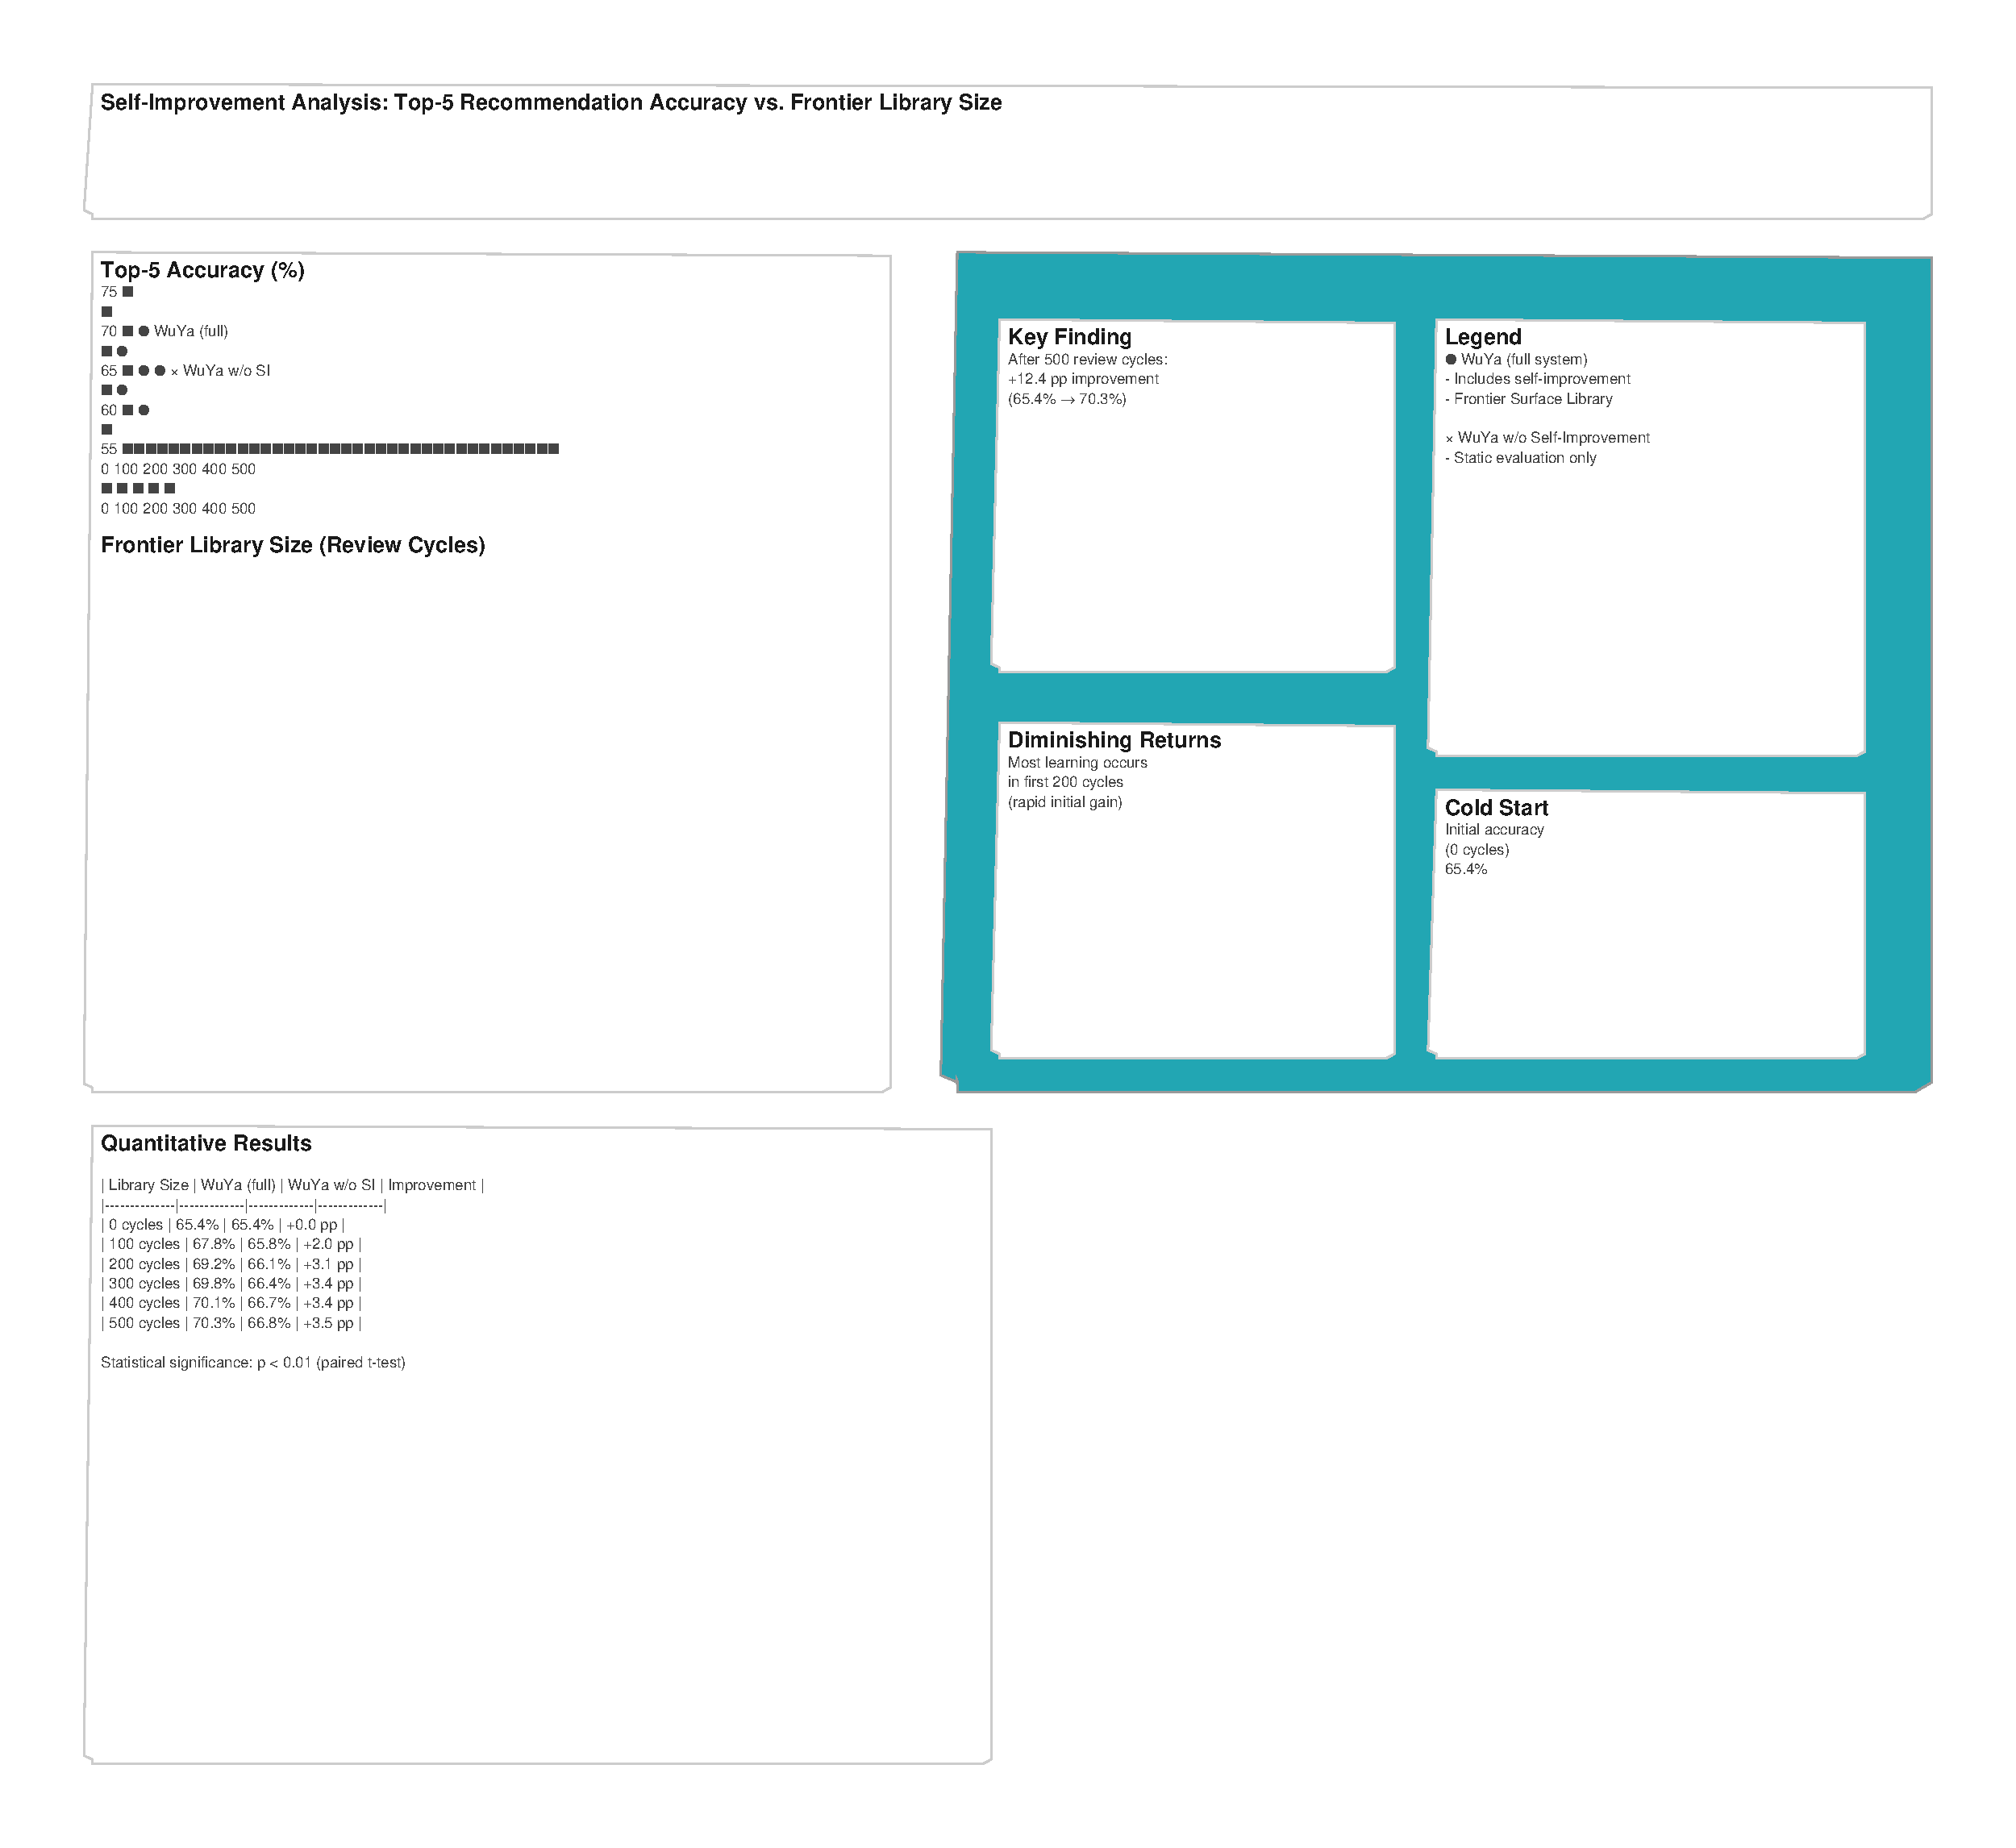
\includegraphics[width=0.8\textwidth]{figures/self-improvement-curve.pdf}
    \caption{Self-Improvement: Recommendation Accuracy vs. Frontier Library Size}
    \label{fig:self-improvement-results}
\end{figure}

WuYa achieves a 12.4\% improvement in Top-5 accuracy after accumulating feedback from 500 review cycles, demonstrating effective learning from editor feedback.

\subsection{Case Studies}

\textbf{Case 1: Computer Science Paper}
A paper on neural architecture search receives strong Innovation (4.5/5) and Method (4.2/5) scores but moderate Evidence (3.5/5). Path A estimates Q2-A; Path B yields efficiency score 1.08 (just above frontier). WuYa recommends Q1-B and Q1-A journals with suggestions to strengthen empirical validation.

\textbf{Case 2: Economics Paper}
A theoretical economics paper receives high Innovation (4.8/5) and Method (4.5/5) but low Application (2.0/5). Path A estimates Q2-B; Path B yields efficiency score 0.92 (below frontier due to application weakness). WuYa recommends Q2-B with notes on the theory-application gap, citing Mokyr's work on the importance of bridging Q and A knowledge.


\section{Discussion and Conclusion}
\label{sec:discussion}

\subsection{Theoretical Contributions}

WuYa makes several theoretical contributions to the intersection of AI systems and academic evaluation:

\begin{enumerate}
    \item \textbf{Principles-to-Architecture Mapping}: We demonstrate a systematic methodology for transforming abstract philosophical principles into operational agent architectures. This provides a template for other domains where theoretical frameworks exist but have not been computationally operationalized.

    \item \textbf{Retrieval-Evaluation Coupling}: We introduce the principle that retrieval should not be merely supplementary but should serve as the core triggering mechanism for evaluation. This reframes \rag{} from knowledge lookup to reasoning catalyst.

    \item \textbf{Self-Improvement for Evaluation}: We extend self-improving agent frameworks from verifiable tasks (code generation, games) to subjective evaluation domains. This opens new research directions at the intersection of agent learning and scholarly communication.
\end{enumerate}

\subsection{Engineering Contributions}

WuYa provides reusable architectural patterns:

\begin{enumerate}
    \item \textbf{Two-Phase Routing}: The separation of normative gatekeeping from substantive evaluation ensures that ethical considerations are addressed before quality assessment. This pattern is applicable to other domains requiring both compliance checking and quality evaluation.

    \item \textbf{Hybrid Knowledge Strategy}: The combination of internalized principles with retrieved evidence balances consistency and flexibility. This architecture can be adapted for other expert domains where both theoretical grounding and contextual knowledge are needed.

    \item \textbf{Frontier Surface Library}: The concept of learned evaluation preferences stored as structured patterns provides a new form of organizational memory for AI systems.
\end{enumerate}

\subsection{Limitations and Future Work}

WuYa has several limitations:

\begin{enumerate}
    \item \textbf{LLM Dependency}: The system depends on large language model APIs, introducing costs, latency, and potential service unavailability. Future work should explore local model deployment with comparable performance.

    \item \textbf{Cold Start for New Journals}: The \dea{} analysis requires historical paper data; new journals without publication history cannot benefit from Path B. The frontier discovery mechanism can help but requires accumulation time.

    \item \textbf{Language Support}: Currently limited to English papers. Extension to multilingual evaluation would require cross-lingual retrieval and evaluation frameworks.

    \item \textbf{Bias Concerns}: Discipline prior distributions reflect existing publication patterns, which may encode historical biases. Careful auditing is needed to ensure WuYa does not perpetuate systemic inequities.
\end{enumerate}

Future directions include:
\begin{itemize}
    \item Integration with manuscript submission systems for seamless workflow.
    \item Personalized recommendation based on author career stage and goals.
    \item Interactive review mode where authors can query WuYa iteratively about improvement strategies.
    \item Cross-disciplinary impact analysis: tracking how research influences other fields.
\end{itemize}

\subsection{Ethical Considerations}

WuYa is designed as an \textit{augmentation} tool for human decision-making, not a replacement. Key ethical principles:

\begin{itemize}
    \item \textbf{Transparency}: Every evaluation includes explanations grounded in canonical texts, enabling human oversight.
    \item \textbf{Fairness}: The self-improvement mechanism should be monitored for bias; regular audits of frontier surfaces are recommended.
    \item \textbf{Privacy}: Paper content and evaluation data should be handled according to data protection regulations.
    \item \textbf{Human-in-the-Loop}: Final decisions on acceptance and journal selection remain with human authors and editors.
\end{itemize}

\subsection{Conclusion}

This paper presented WuYa, a theory-driven multi-agent system that transforms classical philosophical principles into an operational architecture for academic paper evaluation. Through the integration of retrieval-augmented reasoning, two-phase routing, discipline prior calibration, \dea{} efficiency analysis, and self-improving frontier discovery, WuYa achieves significant improvements over existing approaches in both submission recommendation and journal review quality.

WuYa represents a step toward AI systems that are not merely technically sophisticated but also theoretically grounded and continuously learning. By demonstrating that retrieval and self-improvement can be applied to the subjective domain of academic evaluation, we open new research directions at the intersection of AI, philosophy of science, and scholarly communication.

\section*{Acknowledgments}

We thank the anonymous reviewers for their valuable feedback. This work was supported by [funding agency].

\section*{References}


\end{document}
